\documentclass{beamer}
\usepackage{amsmath}
\usepackage{hyperref}
\usepackage{listings}
\usepackage{xcolor}
\hypersetup{colorlinks=true, citecolor=blue, filecolor=blue, linkcolor=blue, urlcolor=blue}
\definecolor{codegreen}{rgb}{0,0.6,0}
\definecolor{codegray}{rgb}{0.5,0.5,0.5}
\definecolor{codepurple}{rgb}{0.58,0,0.82}
\definecolor{backcolour}{rgb}{0.95,0.95,0.92}
 
\lstdefinestyle{mystyle}{
    backgroundcolor=\color{backcolour},   
    commentstyle=\color{codegreen},
    keywordstyle=\color{magenta},
    numberstyle=\tiny\color{codegray},
    stringstyle=\color{codepurple},
    basicstyle=\ttfamily\footnotesize,
    breakatwhitespace=false,         
    breaklines=true,                 
    captionpos=b,                    
    keepspaces=true,                 
    %numbers=left,                    
    numbersep=5pt,                  
    showspaces=false,                
    showstringspaces=false,
    showtabs=false,                  
    tabsize=2
}
 
\lstset{style=mystyle}

\mode<presentation> {

% The Beamer class comes with a number of default slide themes
% which change the colors and layouts of slides. Below this is a list
% of all the themes, uncomment each in turn to see what they look like.

%\usetheme{default}
\usetheme{AnnArbor}
%\usetheme{Antibes}
%\usetheme{Bergen}
%\usetheme{Berkeley}
%\usetheme{Berlin}
%\usetheme{Boadilla}
%\usetheme{CambridgeUS}
%\usetheme{Copenhagen}
%\usetheme{Darmstadt}
%\usetheme{Dresden}
%\usetheme{Frankfurt}
%\usetheme{Goettingen}
%\usetheme{Hannover}
%\usetheme{Ilmenau}
%\usetheme{JuanLesPins}
%\usetheme{Luebeck}
%\usetheme{Madrid}
%\usetheme{Malmoe}
%\usetheme{Marburg}
%\usetheme{Montpellier}
%\usetheme{PaloAlto}
%\usetheme{Pittsburgh}
%\usetheme{Rochester}
%\usetheme{Singapore}
%\usetheme{Szeged}
%\usetheme{Warsaw}

% As well as themes, the Beamer class has a number of color themes
% for any slide theme. Uncomment each of these in turn to see how it
% changes the colors of your current slide theme.

%\usecolortheme{albatross}
%\usecolortheme{beaver}
%\usecolortheme{beetle}
%\usecolortheme{crane}
%\usecolortheme{dolphin}
%\usecolortheme{dove}
%\usecolortheme{fly}
%\usecolortheme{lily}
%\usecolortheme{orchid}
%\usecolortheme{rose}
%\usecolortheme{seagull}
%\usecolortheme{seahorse}
%\usecolortheme{whale}
%\usecolortheme{wolverine}

%\setbeamertemplate{footline} % To remove the footer line in all slides uncomment this line
\setbeamertemplate{footline}[page number] % To replace the footer line in all slides with a simple slide count uncomment this line

\setbeamertemplate{navigation symbols}{} % To remove the navigation symbols from the bottom of all slides uncomment this line
}

\usepackage{graphicx} % Allows including images
\usepackage{booktabs} % Allows the use of \toprule, \midrule and \bottomrule in tables
%\usepackage {tikz}
\usepackage{tkz-graph}
\GraphInit[vstyle = Shade]
\tikzset{
  LabelStyle/.style = { rectangle, rounded corners, draw,
                        minimum width = 2em, fill = yellow!50,
                        text = red, font = \bfseries },
  VertexStyle/.append style = { inner sep=5pt,
                                font = \normalsize\bfseries},
  EdgeStyle/.append style = {->, bend left} }
\usetikzlibrary {positioning}
%\usepackage {xcolor}
\definecolor {processblue}{cmyk}{0.96,0,0,0}
%----------------------------------------------------------------------------------------
%	TITLE PAGE
%----------------------------------------------------------------------------------------

\title[Evolutionary Methods]{Numerical Optimization 11: Evolutionary Methods} %

\author{Qiang Zhu} % Your name
\institute[University of Nevada Las Vegas] % Your institution as it will appear on the bottom of every slide, may be shorthand to save space
{
University of Nevada Las Vegas\\ % Your institution for the title page
\medskip
}
\date{\today} % Date, can be changed to a custom date

\begin{document}

\begin{frame}
\titlepage % Print the title page as the first slide
\end{frame}

\begin{frame}
\frametitle{Overview} % Table of contents slide, comment this block out to remove it
\tableofcontents % Throughout your presentation, if you choose to use \section{} and \subsection{} commands, these will automatically be printed on this slide as an overview of your presentation
\end{frame}

%----------------------------------------------------------------------------------------
%	PRESENTATION SLIDES
%----------------------------------------------------------------------------------------

%------------------------------------------------

\section{Population Methods}
\begin{frame}{Population Methods}
Previous lecture discussed some methods require a group of points to colleHaving a large number of individuals distributed throughout the design space can help the algorithm avoid becoming stuck in a local minimum. Information at different points in the design space can be shared between individuals to globally optimize the objective function. Most population methods are stochastic in nature, and it is generally easy to parallelize the computation. 

These methods typically have the following steps
\begin{itemize}
    \item Initialization
    \item Encoding
    \item Mutation
    \item Crossover
    \item Selection
\end{itemize}

\end{frame}

\section{Initialization}
\begin{frame}{Initialization}
Population methods begin with an initial population, just as descent methods require an initial design point. The initial population should be spread over the design space to increase the chances that the samples are close to the best regions. 
The following strategies can be applied
\begin{itemize}
    \item Uniform distribution in a bounded region
    \item Multivariate normal distribution centered over a region of interest.
    \item The Cauchy distribution has an unbounded variance and can cover a much broader space.
\end{itemize}

\begin{figure}
\centering
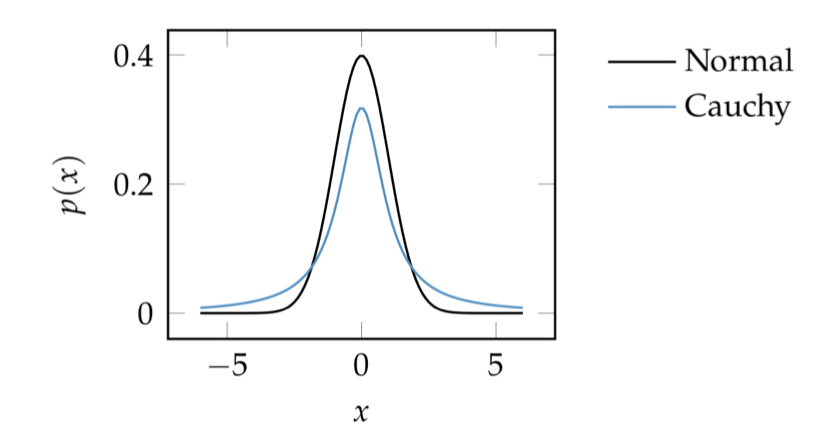
\includegraphics[width=60mm]{Figs/cauchy.jpeg}
\end{figure}   
\end{frame}


\section{Genetic Algorithm}
\begin{frame}{Chromosomes}
There are several ways to represent chromosomes. The simplest is the binary string chromosome, a representation that is similar to the way DNA is encoded.
\end{frame}

\begin{frame}{Selection}
Selection is the process of choosing chromosomes to use as parents for the next generation. For a population with m chromosomes, a selection method will produce a list of $m$ parental pairs for the m children of the next generation. The selected pairs may contain duplicates.
\begin{itemize}
    \item Truncation, random one from the best $k$ truncation
    \item Tournament, the fittest out of $k$ randomly chosen
    \item Roulette wheel, chosen with a probability proportional to the fitness
\end{itemize}

\begin{figure}
\centering
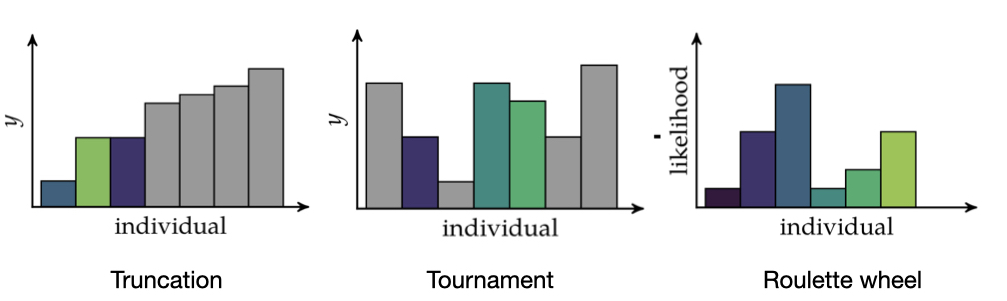
\includegraphics[width=120mm]{Figs/selection.jpeg}
\end{figure}   
\end{frame}

\section{Covariance Matrix Adaptation}
\begin{frame}{Covariance Matrix Adaptation}
Covariance matrix adaptation maintains a mean vector $\boldsymbol{\mu}$, a covariance matrix $\boldsymbol{\Sigma}$, and an additional step-size scalar $\delta$. The covariance matrix only increases or decreases in a single direction with every iteration, whereas the step-size scalar is adapted to control the overall spread of the distribution. At every iteration, m designs are sampled from the multivariate Gaussian
\begin{equation*}
    \boldsymbol{x} \sim \mathcal{N} (\boldsymbol{\mu}, \sigma^2 \Sigma)
\end{equation*}

The designs are then sorted according to their objective function values such that $f(x^1) \leq f(x^2) \leq \cdots \leq f(x^m)$. A new mean vector  $\boldsymbol{\mu}^{k+1}$ is formed using a weighted average of the sampled designs:

\begin{gather*}
    \boldsymbol{\mu}^{k+1} \leftarrow \sum_{i=1}^m w_i \boldsymbol{x}^i\\
    \sum_i^m w_i = 1 ~~~~ w_1>w_2>\cdots>w_m>0    
\end{gather*}

\end{frame}


\section{Particle Swarm Optimization}
\begin{frame}{Particle Swarm Optimization}
Particle swarm optimization introduces momentum to accelerate convergence toward minima. Each individual (particle), in the population keeps track of its current position, velocity, and the best position it has seen so far. Momentum allows an individual to accumulate speed in a favorable direction, independent of local perturbations.

\begin{equation*}
\begin{split}
    \boldsymbol{x}^i & \leftarrow \boldsymbol{x}^i + \boldsymbol{v}^i \\
    \boldsymbol{v}^i & \leftarrow w\boldsymbol{v}^i + c_1 r_1 (\boldsymbol{x}_{lbest}^i - x^i) + c_2 r_2(\boldsymbol{x}_{gbest} - x^i)
\end{split}
\end{equation*}

where 
\begin{itemize}
    \item $x_{lbest}$: the current local best locations for the given population
    \item $x_{gbest}$: the global best locations
    \item $w, c_1, c_2$: empirical parameters
    \item $r_1, r_2$: random numbers drawn from $U(0, 1)$
\end{itemize}

\end{frame}

\begin{frame}{PSO search}
\begin{figure}
\centering
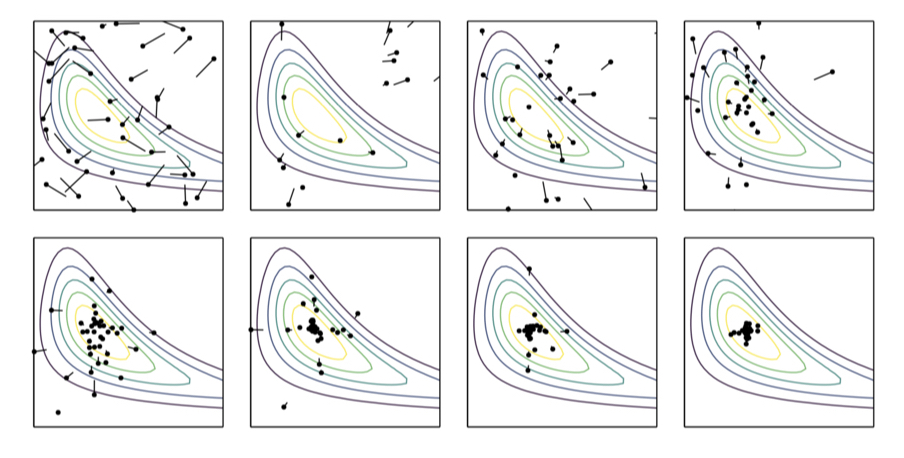
\includegraphics[width=100mm]{Figs/pso.jpeg}
%\caption{Firefly search with $\alpha$ = 0.5, $\beta$ = 1,and $\gamma$ = 0.1 applied to the Branin function}
\end{figure}   
\end{frame}


\begin{frame}{Firefly Algorithm}
The firefly algorithm was inspired by the manner in which fireflies flash their lights to attract mates. In the firefly algorithm, each individual in the population is a firefly and can flash to attract other fireflies. At each iteration, all fireflies are moved toward all more attractive fireflies. A firefly $x_a$ is moved toward a firefly $x_b$ with greater attraction according to

\begin{equation*}
x_a \leftarrow x_a + \beta I (||x_b - x_a||)(x_b - x_a) + \alpha \epsilon
\end{equation*}

where $I$ is the intensity of the attraction and $\beta$ is the source intensity. 
When $\beta$ = 0, it returns to a random walk. where $\epsilon$ is drawn from a zero-mean, unit covariance multivariate Gaussian, and $\alpha$ scales the step size. The resulting update is a random walk biased toward brighter fireflies

The intensity $I$ decreases as the distance $r$ between the two fireflies increases and is defined to be 1 when $r$ = 0. It can be approximated as
\begin{equation*}
    I(r) = e^{-\gamma r^2}
\end{equation*}

\end{frame}

\begin{frame}{Firefly search}
Firefly search with $\alpha$ = 0.5, $\beta$ = 1,and $\gamma$ = 0.1 applied to the Branin function.
\begin{figure}
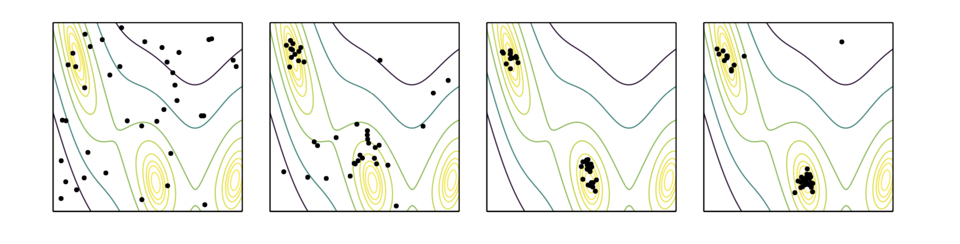
\includegraphics[width=120mm]{Figs/firefly.jpeg}
\end{figure}   

\end{frame}


\section{Summary}
\begin{frame}{Summary}
    \begin{itemize}
        \item Population methods use a collection of individuals in the design space to guide progression toward an optimum.
        \item Genetic algorithms leverage selection, crossover, and mutations to produce better subsequent generations.
        \item Particle swarm optimization and the firefly algorithm include rules and mechanisms for attracting design points to the best individuals in the population while maintaining suitable state space exploration.
        \item Population methods can be extended with local search approaches to improve convergence.
    \end{itemize}
\end{frame}
\end{document}

